\chapter{Annexes}
\label{Annexes}

\section{Redmine}\label{Annexe A}

Redmine est considéré comme l'un des outils de gestion de projets collaboratifs Open Source parmi les plus aboutis. Il recouvre un ensemble de fonctionnalités dont un aperçu est donné ci-dessous, comme la gestion multi-projets, la gestion des demandes d'évolution et des bugs, la gestion et l'indexation des documentations techniques, mais aussi la gestion des droits et des profils des différents intervenants. Il propose aussi une console de suivi de l'état d'avancement des projets, des tâches, des recettes… sous forme de diagramme de Gantt.\\

Redmine est une forge logicielle sous licence GPL. Ses principaux concurrents se nomment Trac, Retrospectiva, Django Projector ou encore InDefero. Notons que Jira ne trouve pas sa place ici, bien qu'il soit le concurrent le plus sérieux de Redmine, parce que Jira est sous Dual licence (l'utilisation commerciale nécessite une licence payante non-Open Source).\\

Redmine offre un ensemble de fonctionnalités comme par exemples :

\begin{itemize}
\item Prise en charge de plusieurs projets
\item Contrôle d'accès avec un modèle flexible de rôles
\item Gestion avancée des tickets
\item Diagramme de Gantt et calendrier
\item Publication de news, documents et gestionnaire de fichiers
\item Notifications par emails et flux ATOM
\item Wiki et forums par projet
\item Outil de suivi du temps
\item Champs personnalisables pour les tickets, suivi de temps, projets et utilisateurs
\item Intégration avec plusieurs SCM : SVN, CVS, Git, Mercurial, Bazaar et Darcs
\item Une communauté active et un ensemble d'outils connexes
\end{itemize}
\\

Plus de détails est disponible sur le wiki du projet : \url{http://www.redmine.org/projects/redmine/wiki}.

\pagebreak

\section{Extraits de codes}\label{Annexe B}\\

\textbf{Instanciation d'un objet upload}\\
\begin{lstlisting}
	// Instanciation
	Upload up = new Upload();
	up.setId(CreateUUID.randomUUID().toString());
	up.setOrganization(user.getOrganization());
	up.setName(fileDetails.getFileName());
\end{lstlisting} \\

\textbf{La classe Upload.java associée}\\

\begin{lstlisting}
	// Empty constructor
	public Upload (){
	}

    // Constructor
    public Upload(String id, String name, String uploadStatus, String organization, String uploadPath){
        super();
        this.id=id;
        this.name = name;
        this.uploadStatus = uploadStatus;
        this.organization = organization;
        this.uploadPath = uploadPath;
    }
    
    // Getters & Setters
    public String getId() {
        return id;
    }

    public void setId(String id) {
        this.id = id;
    }
    
    public String getName() {
        return name;
    }

    public void setName(String name) {
        this.name = name;
    }

    public String getUploadStatus() {
        return uploadStatus;
    }

    public void setUploadStatus(String uploadStatus) {
        this.uploadStatus = uploadStatus;
    }

    public String getOrganization() {
        return organization;
    }

    public void setOrganization(String organization) {
        this.organization = organization;
    }

    public String getUploadPath() {
        return uploadPath;
    }

    public void setUploadPath(String uploadPath) {
        this.uploadPath = uploadPath;
    }
	// suite des Getters & Setters
\end{lstlisting} \\

\textbf{Classe UploadDAO.java}\\

\begin{lstlisting}
	// Create 
    public String create(Upload up)
    {
        System.out.println("Upload instance created : "+up.getId()+" | "+up.getName()+" | "+up.getUploadStatus()+" | "+up.getOrganization()+" | "+up.getUploadPath());
        return persist(up).getId();
    }

    // Read one
    public Upload findByID(String id)
    {
        //return get(id);
        Query query = namedQuery("com.mobigis.dao.Upload.findByID");
        query.setParameter("id", id);
        List<Upload> res = list(query);
        if(res != null && res.size()>0)
        {
            return res.get(0);
        }
        return null;
    }
\end{lstlisting} \\


\textbf{Extrait du log Eclipse}\\

\begin{lstlisting}

INFO  [2015-06-11 15:31:52,883] com.mobigis.thread.AbstractUploadManagerThread: GTFS validation JSON report done !
file unzip : agency.txt
file unzip : calendar.txt
file unzip : calendar_dates.txt
file unzip : fare_attributes.txt
file unzip : fare_rules.txt
file unzip : frequencies.txt
file unzip : routes.txt
file unzip : shapes.txt
file unzip : stop_times.txt
file unzip : stops.txt
file unzip : trips.txt
Extract Done
Clean directory Done
upload status = UPLOADED
INFO  [2015-06-11 15:31:52,920] com.mobigis.thread.AbstractUploadManagerThread: Process upload to Location = C:\mobianalystserver\download\tisseo\gtfs\215b8557-f7c9-4b06-aced-f79bde953c65
INFO  [2015-06-11 15:31:52,920] com.mobigis.thread.AbstractUploadManagerThread: Upload file done ! Id = 215b8557-f7c9-4b06-aced-f79bde953c65 | Status = UPLOADED
C:\mobianalystserver\download\tisseo\gtfs\215b8557-f7c9-4b06-aced-f79bde953c65
INFO  [2015-06-11 15:31:52,965] org.hibernate.engine.internal.StatisticalLoggingSessionEventListener: Session Metrics {
    36877 nanoseconds spent acquiring 1 JDBC connections;
    0 nanoseconds spent releasing 0 JDBC connections;
    358836 nanoseconds spent preparing 4 JDBC statements;
    6286839 nanoseconds spent executing 4 JDBC statements;
    0 nanoseconds spent executing 0 JDBC batches;
    0 nanoseconds spent performing 0 L2C puts;
    0 nanoseconds spent performing 0 L2C hits;
    0 nanoseconds spent performing 0 L2C misses;
    24185654 nanoseconds spent executing 1 flushes (flushing a total of 2 entities and 2 collections);
    42650 nanoseconds spent executing 1 partial-flushes (flushing a total of 0 entities and 0 collections)
}
127.0.0.1 - - [11/Jun/2015:15:31:50 +0000] "POST /upload/gtfs HTTP/1.1" 200 61 "-" "Apache-HttpClient/4.1.1 (java 1.5)" 2254
\end{lstlisting} 

\pagebreak

\section{Structure d'une application Web}\label{Annexe C}\\

\begin{figure}[!h]
\centering
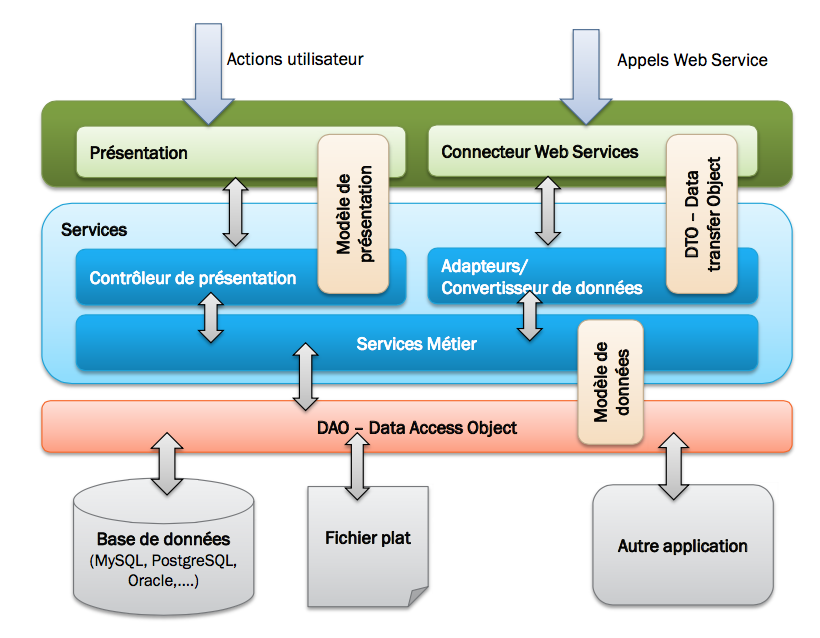
\includegraphics[width=\textwidth]{images/WebAppArchitecture.png}
\caption{\label{WebAppArchitecture}Structure typique d'une application Web}
\end{figure} 

